

%! TeX program = lualatex

% {}\documentclass[a4paper]{article}
% {}\documentclass[a4paper,landscape]{article}
{}\documentclass[a4paper,landscape,twoside]{article}

%-----------------------------------------------------------------
% GENERAL PACKAGES
%-----------------------------------------------------------------
\RequirePackage[ddmmyyyy]{datetime} % change date format
\renewcommand{\dateseparator}{.} % select date separator character
\RequirePackage[shortlabels]{enumitem} % pause/resume lists
\RequirePackage{multicol} % multi column format
\RequirePackage{graphicx} % used for figures
\RequirePackage[dvipsnames]{xcolor} %colors, dvips -> extra premade colors
\RequirePackage[explicit]{titlesec} % formating of titles
\RequirePackage{siunitx} % SI units
\usepackage{amsmath, amssymb} % For mathematical symbols and equations
\RequirePackage{mathtools} % even more math stuff
\RequirePackage{subcaption}
\RequirePackage[hidelinks]{hyperref} % used for hyperlinked nodes
\RequirePackage[document]{ragged2e} % left ragged text
\RequirePackage{atbegshi}  % special commands that apply tikz to all pages
\RequirePackage{etoolbox} % Boolean and if/else
\RequirePackage{calc} % math inside other commands
\RequirePackage{booktabs}
\usepackage{float} % For [H] specifier
\usepackage{parskip} % For paragraph spacing
\usepackage{longtable}
%-----------------------------------------------------------------
% FONT
%-----------------------------------------------------------------
\usepackage{fontspec}
\usepackage[ngerman]{babel}
% \babelfont{rm}{Lato}
\babelfont{rm}{Roboto}
% \babelfont{rm}{Roboto Condensed}
\babelprovide[onchar=ids fonts]{russian}
\babelfont[russian]{rm}{Roboto Condensed}
\babelprovide{english}
%-----------------------------------------------------------------
% GEOMETRY
%-----------------------------------------------------------------
\RequirePackage[
	paperheight=297mm,
	paperwidth=210mm,
	top=3mm,
	bottom=3mm,
	footskip=0mm,
	inner=3mm,
	outer=3mm,
	centering
]{geometry}
%-----------------------------------------------------------------
% OTHER FORMATTING
%-----------------------------------------------------------------
\pagestyle{empty}

%-----------------------------------------------------------------
\usepackage[skip=0.2mm]{caption} % Reduces space between image and caption
\captionsetup{font={footnotesize,sf}}
%-----------------------------------------------------------------
\setlength{\intextsep}{0.2mm} % Space above/below in text
\setlength{\textfloatsep}{0.2mm} % Space between floats
\setlength{\floatsep}{0.2mm} % Space between floats
% -----------------------------------------------------------------
\usepackage{sectsty}
\setcounter{secnumdepth}{1} % Number subsections (##)
% -----------------------------------------------------------------
% space around title and fontsize
\makeatletter
\renewcommand{\section}{\@startsection{section}{1}{\z@}%
	{.5mm}% % Space before
	{.5mm}% % Space after
	{\normalfont\normalsize\bfseries}}
	% {\normalfont\normalsize\bfseries\color{RoyalBlue}}}
\renewcommand{\subsection}{\@startsection{subsection}{2}{\z@}%
	{.25mm}%
	{.25mm}%
	{\normalfont\small\bfseries}}
	% {\normalfont\small\bfseries\color{RoyalBlue}}} % Add color to subsection
\makeatother
% -----------------------------------------------------------------
%indent for paragraph
\setlength{\parindent}{0mm}
% %space between paragraphs
\setlength{\parskip}{0mm}
%space between columns
\setlength{\columnsep}{3mm}
% create lines between columns and define color of columns
% \setlength{\columnseprule}{.3mm} %set thickness default 1pt
% \def\columnseprulecolor{\color{RoyalBlue!20}}
% spacing within lists
\setlist{itemsep=0mm, topsep=0mm} % For all itemize/enumerate
\setlist[itemize]{itemsep=0pt, leftmargin=3mm}
\setlist[enumerate]{itemsep=0pt, leftmargin=4mm}
%-----------------------------------------------------------------
\renewenvironment{quote}
{\list{}{\rightmargin0mm\leftmargin0mm}
	\item\relax\centering\arraybackslash}
% {\endlist\vspace{0mm}} % Adjust 10mm to desired spacing
{\endlist\vspace{-1mm}} % Adjust 10mm to desired spacing
%-----------------------------------------------------------------
% INHALT
%-----------------------------------------------------------------

\begin{document}

\begin{multicols}{4}

	\begin{center}
		%-----------------------------------------------------------------
		\LARGE \textbf{\colorbox{RoyalBlue}{\textcolor{white}{Strategische Studien II}}} \\
		\normalsize
		\textbf{\colorbox{lightgray}{\textcolor{Black}{Stadelmann Silvan} \url{silvasta@ethz.ch}}}\\
		\today{}
		%-----------------------------------------------------------------
	\end{center}

	% The column width is: \the\columnwidth
	% parskip is: \the\parskip{}
	% Militärakademie (MILAK) an der ETH Zürich\\
	% Vorlesung Strategische Studien II\\
	% Dr.~Marcel Berni\\

	\footnotesize

	\section{Einleitung}
	\begin{figure}[H]
		\centering
		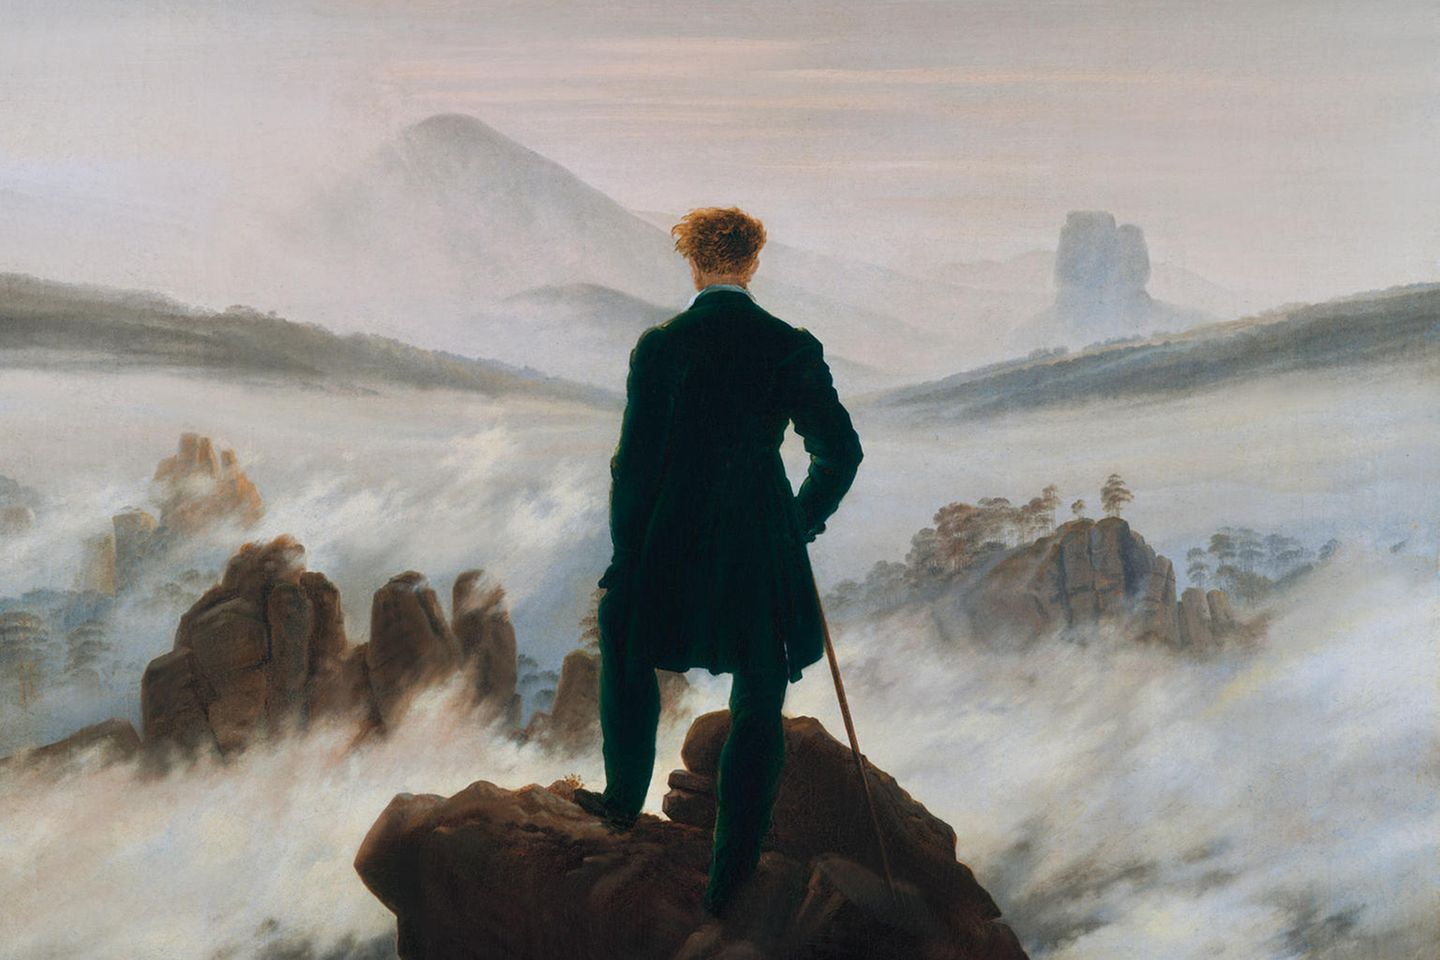
\includegraphics[width=.7\columnwidth]{images/wanderer.jpg}
		\caption*{\centering
			Der Wanderer über dem Nebelmeer

			Caspar David Friedrich, 1818
		}
	\end{figure}

	\subsection{Strategie, Operation und Taktik}

	\begin{quote}
		Mit Taktik gewinnt man das Gefecht, mit Operationen einen Feldzug und
		mit Strategie einen Krieg.
		- \emph{Gustav Däniker, Schweizerische Selbstbehauptungsstrategie im
			Kalten Krieg, Frauenfeld 1996}
	\end{quote}

	\subsection{Gray, Modern Strategy, 17 Dimensionen}

	\begin{quote}
		Overall, strategy is where policy meets the battlespace {[}\ldots{]} On
		the strategy bridge, the strategist must translate political desires
		into plans for their realization. {[}\ldots{]} Strategy is only the
		bridge connecting the world of tactical engagement with that of
		political purpose.

		\emph{Colin S. Gray, Westport-London 2007}
	\end{quote}

	\begin{itemize}
		\item
		      Krieg und Strategie als ganzheitliches Phänomen
		\item
		      Dimensionen zeitlos gültig aber Wirkung variiert
		\item
		      Exzellenz in allen Dimensionen nicht notwendig
		\item
		      Dramatische Verbesserung in einem oder zwei Bereichen garantieren
		      keinen strategischen Erfolg
		\item
		      Katastrophale Schwäche in einer kann tödlich sein
	\end{itemize}

	\vspace{.4mm}
	\textbf{People and Politics}
	People,
	Society,
	Culture,
	Politics,
	Ethics
	\textbf{  Preparation of War}
	Economics and Logistics,
	Organization (incl. Defence and Force Planning),
	Military administration (incl. Recruitment, Training, Armaments),
	Information an Intelligence,
	Strategic Theory an Doctrine,
	Technology
	\textbf{ War Proper}
	Military Operations,
	Command,
	Geography,
	Friction,
	Adversary,
	Time

	\subsection{Mittel, Methoden und Ziele}

	\begin{quote}
		Strategy equals ends (objectives toward which one strives) plus ways
		(courses of action) plus means (instruments by which some end can be
		achieved).\\
		\emph{Arthur F. Lykke, 1984--1985}
	\end{quote}

	\subsection{Modernes Strategieverständnis}

	Wie erreicht man seine Ziele gegen einen Gegner?

	\begin{itemize}

		\item
		      (Politische) Festlegung und Verfolgung eines Ziels
		\item
		      Formulierung und Anwendung eines Plans, unter Berücksichtigung des
		      Gegners und Hindernisse
		\item
		      Einsatz offener und verdeckter Mittel und Methoden
		\item
		      Erfolgsmassstab: abhängig von Beobachter und Zeit
	\end{itemize}

	\begin{quote}
		\textbf{Eine Strategie ist ein Plan über den Mitteleinsatz zur
			Zielerreichung unter Berücksichtigung der gegnerischen Strategie sowie
			externer Faktoren.}
	\end{quote}

	\section{Joint Warfare}

	\textbf{Begriffe}
	CrossDomain Operations,
	Integrated Operations,
	Comprehensive Approach,
	Distributed Operations,
	Cyber-physical Operations,
	Full spectrum warfare
	\textbf{Effects-based Operations}
	\textit{Bild Kopernikus}
	Vergleich mit Entdeckung der tatsächlichen funktionsweise der Umlaufbahn.
	\textbf{Network-centric Warfare und Effects-based Operations}
	Effekte - Systemanalyse - Wahl der Mittel aus gesamtem
	Spektrum, fein dosiert mit Priorisierung der zivilen/psychologischen
	Mittel, Zentrale Stellung in US- und NATO-Doktrinen

	\begin{quote}
		\textbf{Wir definieren die wirkungsraumübergreifende Kriegsführung als
			koordinierte militärische Operationen verschiedener Teilstreitkräfte,
			die zwei oder mehr Operationsräume miteinander verbinden.}
	\end{quote}
	\vspace{.8mm}
	\subsection{Grundlage AirLand Battle (1982/86)}

	\begin{itemize}
		\item
		      Offensive Ausrichtung, Manöver statt Abnutzung
		\item
		      Kampf der verbundenen Waffen, Synchronisierung von: Close/Deep/Rear Operations
		\item
		      Initiative durch Tempo, Überraschung, Täuschung, Flexibilität,
		      Ziel ist Paralysierung des  Gegners
		\item
		      Bezüge zu Clausewitz und Liddell-Hart
		\item
		      Paradebeispiel ``Desert Storm'' (1991)
	\end{itemize}


	\subsection{Multi Domain Operations 2016}

	Neueste Konzeption mit bislang unscharfen Konturen.
	Wirksamkeit gegen Hauptbedrohung bisher wenig erwiesen.
	Stark von amerikanischen Denkern und Technologiegläubigkeit geprägt.
	Neuausrichtung von Aufstandsbekämpfung auf reguläre Gegner.
	\textbf{Unterschied zu JO}
	MDO inkludiert nicht-militärische Assets
	\textbf{Ablauf}
	Penetrate,
	Dis-integrate,
	Exploit,
	Re-compete.

	\section{Geopolitik und Geostrategie}

	\begin{itemize}
		\item
		      Interdisziplinäre Verbindung von Aussen- und
		      Sicherheitspolitik mit Natur- und Geisteswissenschaften
		      (Geografie, Evolutionsbiologie, Geschichte \ldots)
	\end{itemize}
	\begin{quote}
		{[}Geography is{]}... the mother of strategy.\\
		- \emph{Gray/Sloan in Geopolitics, Geography and Strategy,
			London 1999}
	\end{quote}

	\textbf{Heartland Theory}
	Rede Mackinders vor Royal Geographic Society 1904
	\textbf{Rimland Theory}
	Spykman, America's Strategy in World Politics, New York 1942
	\textbf{Grand Chessboard}
	Brzezinski, Game Plan. A Geostrategic Framework for
	the Conduct of the US-Soviet Contest, New York 1986
	\textbf{Kampf der Kulturen}
	Huntington, The Clash of Civilizations 1993 ... and the Remaking of World Order 1996
	\textbf{Geoökonomie und Friend-shoring}
	Fähigkeit, wirtschaftliche Stärke aus
	bestehenden Finanz- und Handelsbeziehungen zu nutzen, um geopolitische
	und wirtschaftliche Ziele zu erreichen.
	\textbf{Lattice-like Security Architecture}
	Hub-and-Spokes Allianzsystem der USA in Asien


	\section{Sowjetische Militärstrategie}

	\textbf{Kutusow} (1745-1813) Russland gewinnt Kriege durch Geduld.
	\textbf{Suworow} (1730- 1800) Russland gewinnt Kriege durch Schnelligkeit.
	\textbf{Frunse} (1885-1925)
	Nächster Krieg langwierig und defensiv,
	Operationsraum wegen weitreichender Mittel riesig,
	Front und Hinterland vernetzen,
	Gesellschaft und Wirtschaft militarisieren,
	wenn nötig direkter Ansatz,
	Ideologische Beeinflussung

	\textbf{Rote Armee} 1928/29 erneut Konzeptionsstreit:

	\begin{itemize}
		\item
		      Abnutzung: Alexander Swetschin 1978-1938
		\item
		      Zerstörung: Wladimir Triandafillow 1987-1931

		      \ \ \ \ \ \ \ \ \ \ \ \ \ \ \ \ \ \ \ Michail Tuchatschewski 1893-1937
	\end{itemize}

	\subsection{Theorie der Operationskunst (Swetschin)}

	\begin{itemize}
		\item
		      Politikfreie operative Kunst, primär defensiv
		\item
		      Drei Stufen: Strategie, (neu) Operation, Taktik
		\item
		      Organisation des Rückraums, Durchhaltefähigkeit
		\item
		      Definition der Operation um Planung und Vorbereitung
		      erweitert, durchgeführt von Militärexperten
	\end{itemize}

	\subsection{Tiefe Operation (Isserson)}

	\begin{itemize}
		\item
		      Von Anfang an offensive Vorgehensweise
		\item
		      Durchbruch mit Feuerkraft und Masse, Wellen
		\item
		      Gestaffelte Aufstellung, Riesiger Kräftebedarf
		\item
		      Unterstützung durch Aufrüstungsprogramm Stalins
		\item
		      \textbf{Operation Bagration} als mögliches Beispiel
	\end{itemize}


	\subsection{Reform der Tiefen Operation (Sokolowski)}

	\begin{itemize}
		\item
		      Operationsraum maximiert durch neue Waffen
		\item
		      Krieg muss in Initialphase entschieden werden
		\item
		      Konventionelle Streitkräfte angeblich noch zur Landesverteidigung und in regionalen
		      Kriegen benötigt
	\end{itemize}

	\section{Reguläre vs. irreguläre Kriegführung}

	\textbf{Ius ad bellum} (Recht zum Krieg)
	Mit dem Kriegsverbot von 1945 soll
	''Der Krieg ist eine blosse Fortsetzung der Politik mit anderen Mitteln''
	aufgegeben werden.
	\textbf{Ius in bello} (Recht im Krieg)
	Humanitäres Völkerrecht oder Kriegsrecht regelt, was im Krieg zulässig ist.
	\begin{itemize}
		\item
		      Krieg völkerrechtlich geächtet, das moderne Völkerrecht
		      spricht nur noch von bewaffnetem Konflikt.
		\item
		      Krieg als hochkomplexes Phänomen lässt sich nicht mit
		      einfachen Formeln alt/neu, (un)konventionell, (a)symmetrisch,
		      (ir)regulär, hybrid kategorisieren.
		\item
		      Wir unterscheiden zwischen (ir-/)regulärem Krieg
	\end{itemize}

	\textbf{Krieg} Anwendung organisierter bewaffneter Gewalt zwischen
	menschlichen Kollektiven zur Durchsetzung von Interessen und mit Folge
	von Todesopfern und physischen Schäden
	\textbf{Regulärer Krieg} meint den Krieg zwischen zwei (oder mehr)
	Staaten
	\textbf{Irregulärer Krieg} meint den Krieg zwischen einem (oder
	mehreren) Staaten einerseits und einer (oder mehrerer)
	nicht-staatlicher Gruppierungen andererseits.

	\subsection{Regulärer Kombattant}

	\begin{enumerate}
		\def\labelenumi{\arabic{enumi}.}
		\item
		      dass jemand an ihrer Spitze steht, der für seine Untergebenen
		      verantwortlich ist,
		\item
		      dass sie ein bestimmtes, aus der Ferne, erkennbares Abzeichen tragen,
		\item
		      dass sie die Waffen offen führen und
		\item
		      dass sie bei ihren Unternehmungen die Gesetze und Gebräuche des
		      Krieges beobachten.
	\end{enumerate}

	\section{Aufstandstheorien}

	\subsection{Generelle Aufstandsstrategie}

	\begin{itemize}
		\item
		      Keine Suche nach Entscheidungsschlacht, stattdessen Überdehnung Gegner
		\item
		      Hohe Kosten für Gegner (materiell, aber auch politische Legitimität)
		      provozieren
		\item
		      Unterstützung durch Bevölkerung entscheidend (aktive Minderheit und
		      passive Mehrheit)
		\item
		      Schrittweiser Übergang zu direkterer Konfrontation
	\end{itemize}

	\subsection{Sozialrevolutionärer Aufstand}

	\begin{itemize}
		\item
		      Engels: Organisation, Entschlossenheit, Momentum
		\item
		      Mao: Drei Phasen des Volkskrieges, seriell:

	\end{itemize}
	Defensive: Aufbau Organisation, Rekrutierung
	- Gleichgewicht: begrenzte Angriffe aus sicherem Gebiet
	- Offensive: mit disziplinierter, regulärer Armee
	- Kampf primär politisch (Analyse Beziehung Partisanen-Volk)
	\begin{itemize}
		\item
		      Che: Gewalt durch Avantgarde transformiert politische Situation,
		      Proliferation von Focos
	\end{itemize}

	\subsection{Ethnisch-nationalistischer Aufstand}

	\begin{itemize}

		\item
		      von Dach: Umfassende Aufstandstheorie, Volksaufstand im Kriegsfall, Rückgriff auf Besonderheiten
		      der Schweiz, Idealisierung der Opferbereitschaft, Unterschätzung
		      Risiken/Missbrauchspotenzial
	\end{itemize}


	\subsection{Islamistischer Aufstand}
	\begin{itemize}

		\item
		      Suizidattentat und Terrorismus
		\item
		      Diskrepanz Theorie - Realität (Umsetzung)
	\end{itemize}


	\subsection{Externe Unterstützung als Erfolgsfaktor?}

	\begin{itemize}
		\item
		      Verbesserte militärische Fähigkeiten, Informationen, Ressourcenzuwachs, politische
		      Anerkennung
		\item
		      Potenziell signifikante Kosten und Risiken möglich
	\end{itemize}

	\section{Aufstandsbekämpfungstheorien}


	\begin{itemize}

		\item
		      Konventionelle Kriegführung gegen irregulären Gegner
		      nicht erfolgversprechen, häufig Unterschätzung
		\item
		      Erfolgsbilanz schlecht, politischer Wille für COIN tief
		\item
		      COIN-Erfolg abhängig von Verhältnissen im Zielland: Regierung muss
		      Legitimität bei Bevölkerung schaffen
		\item
		      Population Centric Approach \textless---\textgreater{} Kinetic Approach
	\end{itemize}


	\textbf{Maximal Force}
	Callwell (1859-1928)
	Lessons to Be Learned from the Campaigns in Which British Forces
	Have Been Employed, 1887 -
	Small Wars: Their Principles and Practice, 1896-1906
	\textbf{Minimal Force}
	Gwynn (1870-1962)
	Imperial Policing 1934
	\textbf{Malayan Emergency (1948-1960)}
	Aufbau multiethnische malaiische Armee/Polizei/Regierung.
	\textbf{Algerienkrieg (1954-1962)}
	Front de Libération Nationale (FLN) vs.
	Französische Armee
	\textbf{Die französische Doktrin}
	Roger Trinquier (1908-1986)
	David Galula (1919-1967)
	schlussfolgern, dass es nach der
	Niederlage bei Dien Bien Phu (1954) eine neue Doktrin brauche.

	\subsection{Technologie und COIN in Vietnam
		1965-1975}

	\begin{figure}[H]
		\centering
		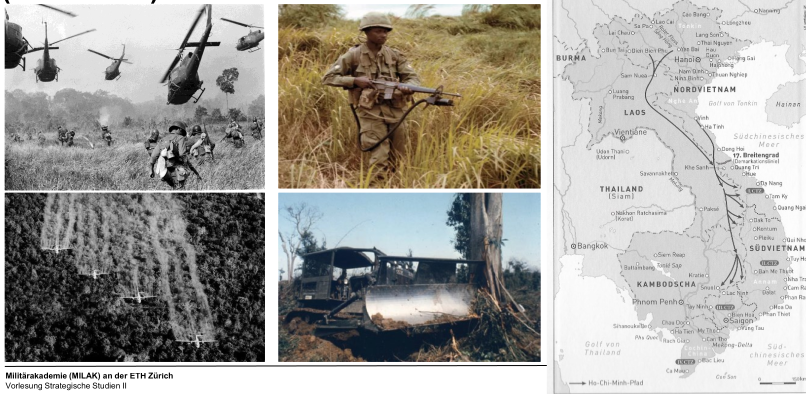
\includegraphics[width=\columnwidth]{images/vietnam.png}
		\caption{
			Luftaufklärung (links,o)
			Agent Orange (links,u)
			Schnüffelgerät (mitte,o)
			Abholzung (mitte,u)
			Versorgung durch \textbf{Ho-Chi-Minh-Pfad} (rechts)
		}
	\end{figure}


	\section{Strat. Bedeutung Kriegsgefangener}

	\begin{itemize}

		\item
		      Mannigfaltige strat. Bedeutungen Kriegsgefangener: Vom
		      Informationsträger über die politische und diplomatische Symbolik bis
		      zur Verhandlungsmasse
	\end{itemize}

	\textbf{General Orders No.100 1863}
	US Civil War,
	Kriegsgefangenschaft als Schutz-, nicht Strafmassnahme,
	\textbf{1871}
	Unvorstellbare Anzahl POWs,
	Regulativ über Behandlung und Verpflegung,
	erstmals Involvierung int. Organisationen.
	\textbf{Haager Landkriegsordnung}
	Konferenzen 1899/1907,
	Grundsatz: Unbedingte Verschonung sich ergebender Gegner und angemessene Behandlung


	\textbf{Genfer Konvention 1929}
	Bis dato umfassendste Kodifikation,
	Völkerrechtliche Akzeptanz des IKRK
	\textbf{Neuauflage 1949}
	Anpassung  nach WW2
	\textbf{Zusatzprotokolle}
	Verbietet insbesondere Tötung, Gefährdung, Gewaltanwendung, Folter,
	Verstümmelung, Experimente, Bedrohung, Beleidigung, Erniedrigung,
	öffentliches Zurschaustellen, Repressalien sowie Vergeltungsmassnahmen

	\subsection{Wer bekommt Kriegsgefangenenstatus?}

	Reguläre Kombatanten,
	Milizen und Freiwilligenkorps,
	wenn sie die Regeln für reguläre Kombatanten erfüllen.
	\textbf{Info}
	Auch irreguläre Kombattanten müssen als Kriegsgefangene behandelt werden, bis ihnen
	ein Kriegsgericht den Kriegsgefangenenstatus abspricht.

	\subsection{Kriegsgefangene als Informationsquelle}

	Kriegsgefangene müssen nur:
	Name,
	Dienstgrad,
	Geburtsdatum
	und Erkennungsnummer preisgeben.
	Verhöre sind erlaubt, dürfen aber nicht zu Schäden führen.


	\section{Kriegslogistik}

	% \begin{figure}[H]
	% 	\centering{}
	% 	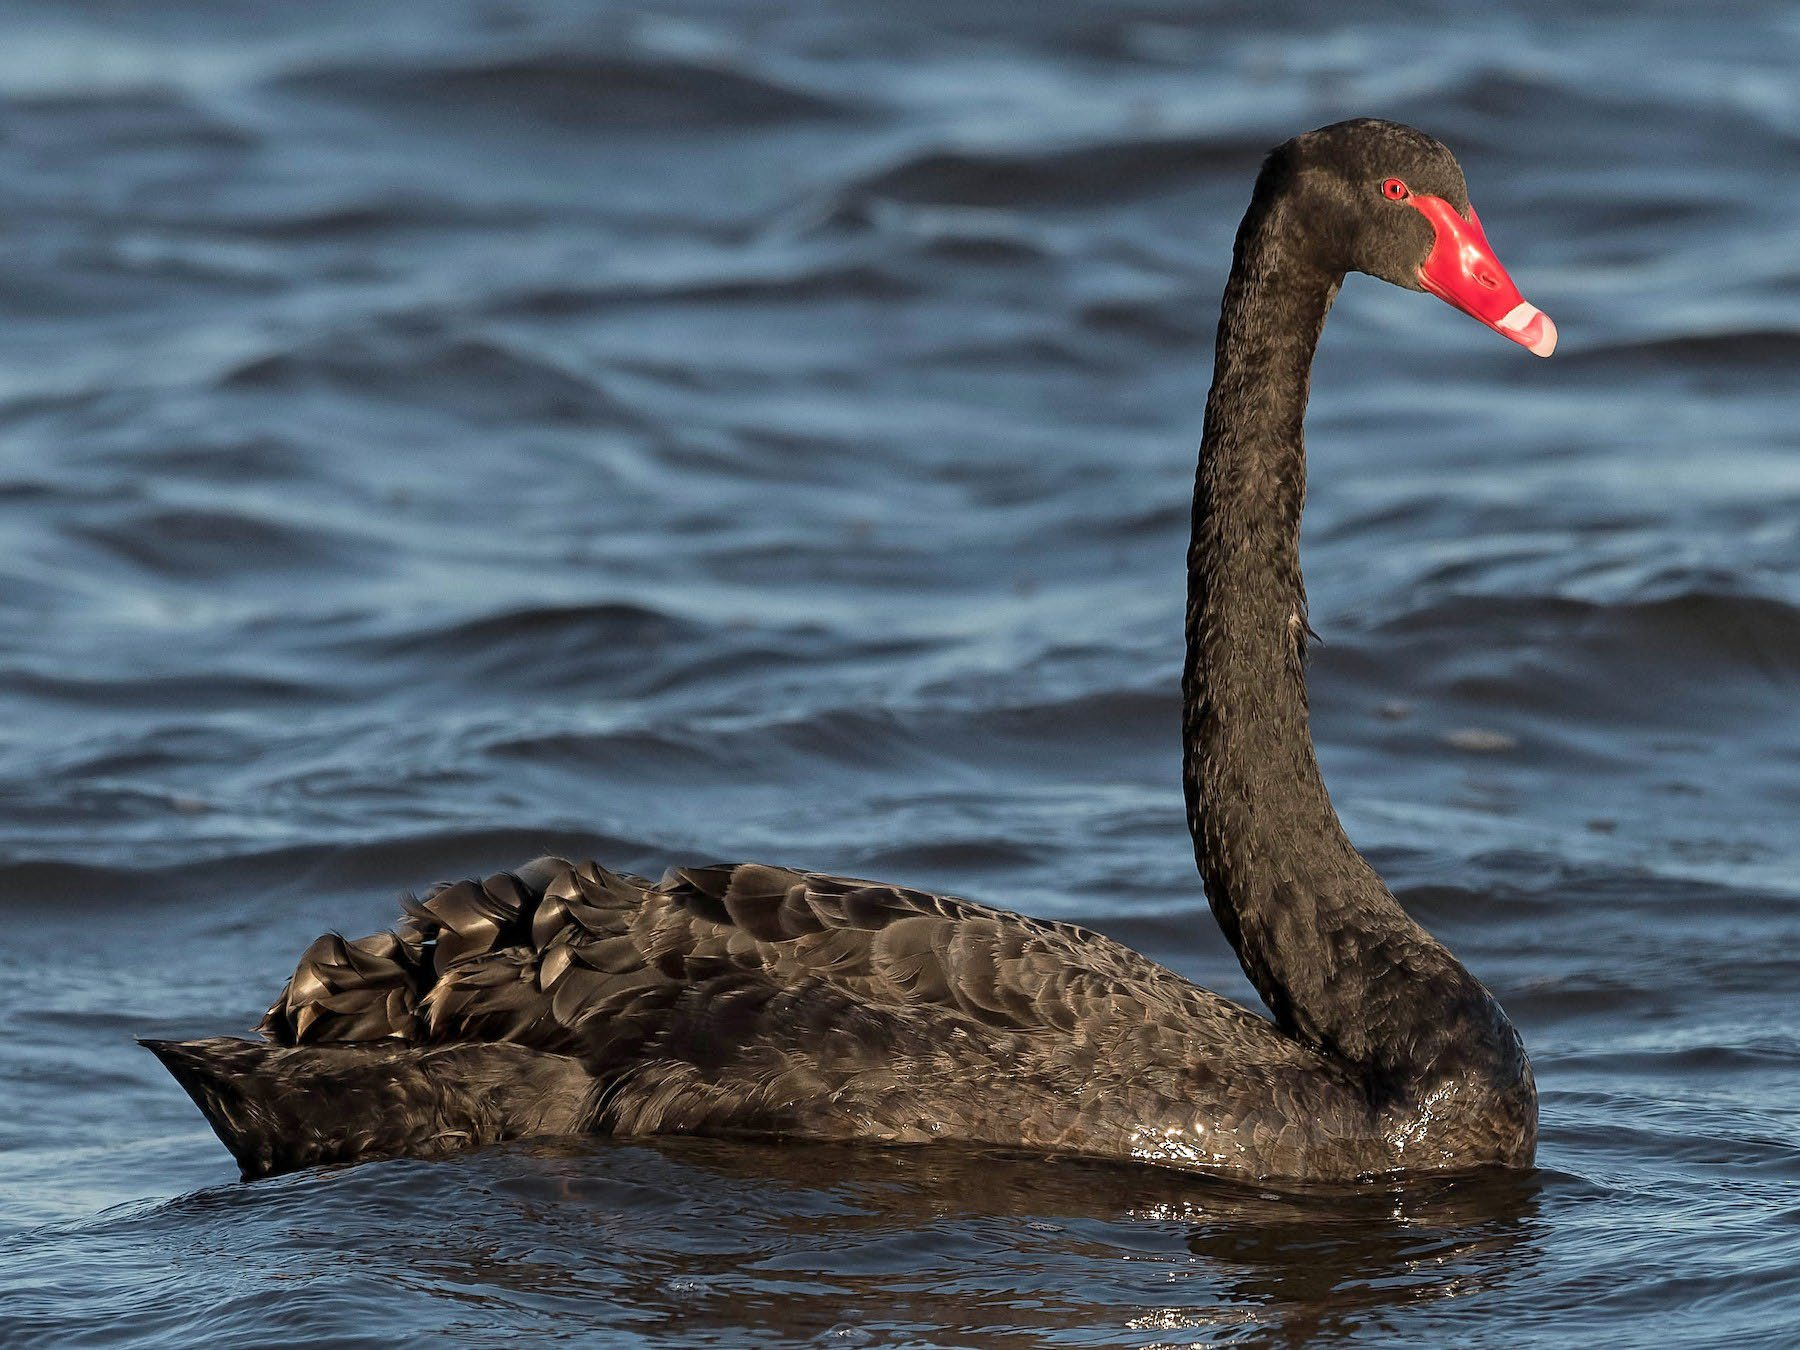
\includegraphics[width=.15\columnwidth]{images/swan.png}
	% 	\caption
	% 	{Be the swan... ?}
	% \end{figure}

	\subsection{5 D der Logistik}

	\textbf{Destination}
	Gute Infrastruktur ist rar,
	Militäringenieure zum Aufbau oder zum Räumen von Gefahren,
	Air Point of Disembarktion (APOD),
	Sea Point of Disembarkation (SPOD),
	Beach
	\textbf{Distance}
	Kommunikationslinien (LOC) können lang werden.
	Risiko Management, was ist akzeptierbar?
	\textbf{Demand}
	Push in Anfangsphase, besonders Treibstoff und Munition,
	Pull bei Personalsupport, Medizinische Versorgung
	\textbf{Wasser}
	Grundwasser reinigen,
	Gesundheitsschutz, Benötigt medizinische Infrastruktur.
	\textbf{Duration}
	Aufrechterhaltung von Standort benötigt Planung von:
	Personal,
	Zulieferer,
	\textbf{Dependency}
	Verträge mit externen  Zulieferern, Dienstleistern weit verbreitet,

	\subsection{Fünf Lektionen aus der Ukraine}

	\textbf{1 - Tactical and operational effects of UAS}

	(Glasfaser/Autonome) \textbf{Drohnen}
	Trefferquote 10-80\% (nicht alle explodieren),
	Je nach Modell anfällig auf Signalstörung.
	\textbf{Operational level systems}
	Bayraktar TB2,
	Harop,
	\textbf{Medium Altitude Long Endurance systems}

	\textbf{2 - Transparent tactical battlespace}

	Tarnnetze reichen nicht, elektronische Signatur,
	Kommandoposten anfällig, viel Wärme und Funkstrahlung.

	\textbf{3 - Need to hide but still exercise C2}

	Kein Hinterland, erhöhte Reichweite und Aufklärung.
	Ständiger Standortwechsel erschwert C2.

	\textbf{4 - Medical support is difficult and has changed}

	Aus der Luft verunmöglicht.
	Blutversorgung von entscheidender Bedeutung,
	\textbf{einfacher Blut vorwärts zu senden als Chirurgie}

	\textbf{5 - Civilian contractors and conflict zones don't mix}

	Contractor Support to Operations (CSO) hat sich seit 2. Golfkrieg
	etabliert und gut funktioniert, \textbf{hier nicht.}

	\section{Der Bergkarabachkonflikt}


	\begin{itemize}

		\item
		      Externe Unterstützung und Ausnutzung von Gelegenheitsfenstern
		      kann kriegsentscheidend sein
		\item
		      Angriffsdrohnen ermöglichten Aserbaidschan die Schwächung der
		      armenischen Verteidigung
		\item
		      Traditionelle Luftverteidigung ist unzureichend, um gegen
		      Angriffsdrohnen bestehen zu können
	\end{itemize}
	\vspace{1mm}
	\textbf{Vorgeschichte}
	Gründung der Republiken GEO, ARM und AZE 1918 -
	Autonome Oblast Bergkarabach \selectlanguage{russian}СССР\selectlanguage{ngerman} (1923-1991)
	Deklaration Autonome Republik Berg-Karabach 1991 (seit 2017 Arzach)
	Erster Bergkarabach-Krieg (1992-1994)
	\textbf{Kriegsursachen}
	Ungelöster Territorialdisput (frozen conflict)
	Militärische Aufrüstung,
	Aussenpolitik Türkei,
	Innenpolitische Spannungen in Aserbaidschan
	\textbf{Kriegsauslöser}
	Grenzscharmützel,
	Militärübungen,
	Provokation von Schuscha
	% \textbf{Gemäss ARM}
	% Offensive AZE, 27.09.2020, 8h03
	% \textbf{Gemäss AZE}
	% ARM Beschuss gn Stellungen, 6h00 deshalb Gegenoffensive

	\textbf{\selectlanguage{russian}ОДКБ \selectlanguage{ngerman}}
	- Militärisches Bündnis um Russland
	- Armenien ist Teil davon
	- Armenien hat sich dem Westen zugewannt
	- Russland hat militärisch nicht interveniert
	(Reihenfolge der letzten zwei Punkte unklar)

	\textbf{Konfliktverlauf}
	27.09.20-10.11.20
	\textbf{Waffenstillstand}
	-  Stadt Schuscha auf Hügel an strategisch wichtiger Lage
	-  Schnelle Einnahme durch Aserbaidschan
	-  Darauffolgend der Waffenstillstand
	\textbf{Rückeroberung Bergkarabach 2023}
	Blockade der Republik Arzach durch AZE -
	AZE bricht Waffenstillstand und greift Republik Arzach an -
	Waffenstillstand unter russischer Vermittlung
	- Flucht von über 100 000 armenischen Zivilisten



	\section{Der Ukrainekrieg}

	Derzeit findet auf der strategischen Ebene ein Abnutzungskrieg statt,
	bei der die Kriegswirtschaft und Unterstützung der Partner  elementar ist.


	\textbf{Anfangsphase 2022}
	Hauptstösse auf vier Angriffsachsen
	\textbf{Strategiewechsel Sommer-Herbst 2022}
	Fokus Donbass
	\textbf{Ukrainische Gegenoffensive 2023}
	Minimale Erfolge, hoher Verlust an Material und Personal
	\textbf{Stellungskrieg 2023}
	Einnahme Bachmut, Vorstoss auf Awdijiwka
	\textbf{Stellungskrieg 2024}
	Einnahme Awdijiwka, darauf Vorstoss Pakrovsk, Chasiv Jar, weitere Städte im Donbass.
	Vorstösse entlang Ostseite Oskil, von Kupjansk bis Liman.
	Abenteuer in Kursk.

	\subsection{Frozen Conflict 2025?}

	Kellog: Sicherheitszone und Truppenstationierung

	\begin{figure}[H]
		\centering
		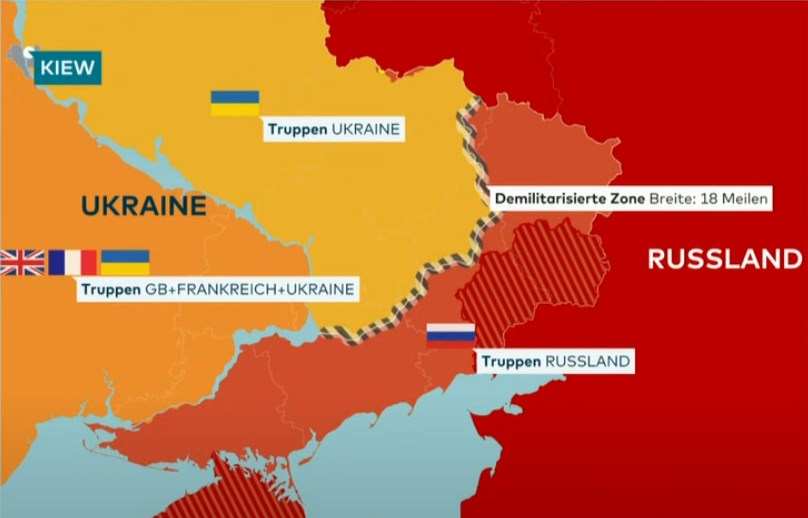
\includegraphics[width=.91\columnwidth]{images/buffer-usa.png}
		\caption{Vorstellung USA}
	\end{figure}
	\begin{figure}[H]
		\centering
		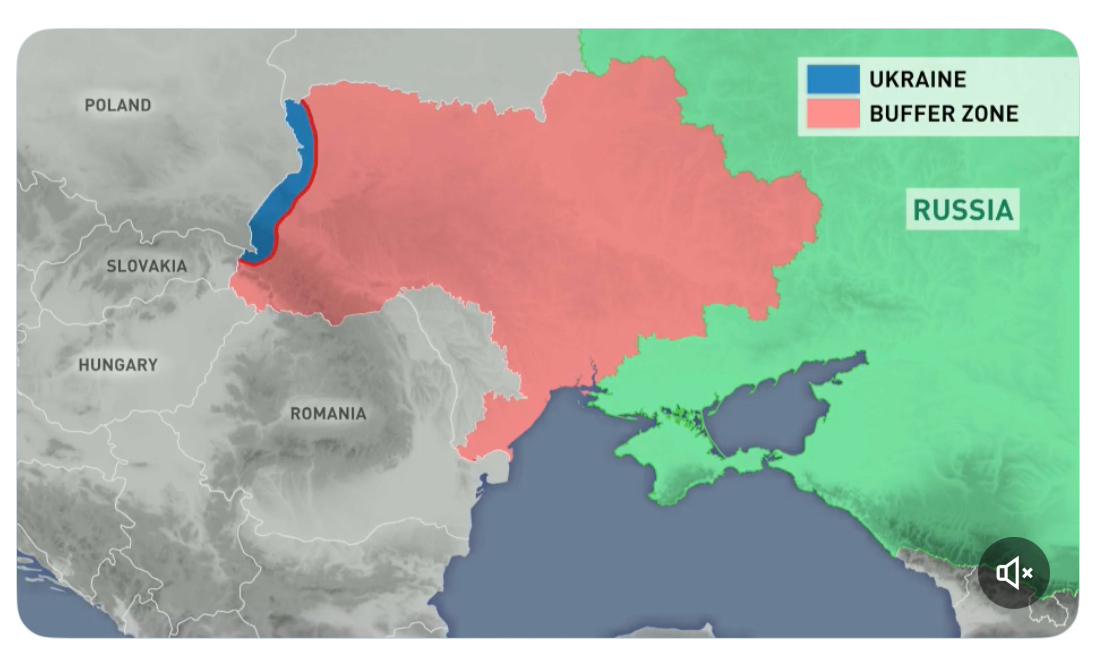
\includegraphics[width=.95\columnwidth]{images/buffer-rf.jpg}
		\caption{Vorstellung Russland}
	\end{figure}


	\subsection{Mögliche Entwicklung}

	Unterstützung der Ukraine hält an,
	Russland geht Munition, Material und qualifiziertes Personal aus
	$\Rightarrow$
	\textbf{Ukraine gewinnt Krieg}
	|
	Russische Gebietsverluste,
	hohe russische Verluste,
	$\Rightarrow$
	\textbf{Sturz des Regimes in Russland}
	|
	Ukraine erleidet Rückschläge,
	Russland erobert weitere Gebiete
	$\Rightarrow$
	\textbf{Waffenstillstand}
	|
	Einstellen der Unterstützung durch den Westen,
	Ukraine geht Munition und Material aus
	$\Rightarrow$
	\textbf{Russland gewinnt Krieg}
	|
	Keiner Seite gelingt ein Durchbruch,
	Beide Seiten halten an Kriegszielen fest,
	$\Rightarrow$
	\textbf{Abnutzungskrieg an langer Frontlinie}

	\section{Israels Mehrfrontenkriege}

	\begin{itemize}
		\item
		      Strategische Kultur der Offensive prägt Israel.
	\end{itemize}

	\textbf{Al-Aqsa Flutwelle}
	Ausschalten von Verteidigungs-, und Überwachungssystemen
	und Vorrücken entlang gesamter Grenzlinie.
	\textbf{Israelische Reaktion}
	SWORDS OF IRON - blutigster Konflikt in Gaza,
	+50k Palästinenser getötet,	mehrheitlich Zivilisten,
	humanitäre Katastrophe.
	\textbf{Ziele Gemäss Regierung}
	Zerstörung Hamas,
	Befreiung Geiseln,
	Wiederherstellung Abschreckungsfähigkeit IDF.

	\textbf{Iran}
	Eliminierungen durch Israel in Syrien, Irak und Iran mit Luftangriffen.
	Massive Raketenangriffe hauptsächlich auf militärische Einrichtungen durch Iran.
	\textbf{Hisbollah}
	Nach 7.10.2023 gegenseitiger Beschuss.
	Nach Pager-Angriff Bombardierungen, Eliminierungen und leichte Bodenoffensive.
	Seit November 2024 unruhiger Waffenstillstand (öfters gebrochen)
	\textbf{Syrien}
	Sturz Bashar al-Assads
	$\Rightarrow$
	Netanyahu erklärt Waffenruhe als gebrochen
	$\Rightarrow$
	Operation Arrow of Bashan:
	Zerstörung syrisches Kriegsmaterial,
	Besetzung demilitarisierter Golanhöhen



	\section{Der syrische Bürgerkrieg}

	Im November/Dezember 2024 gelang es der HTS mit türkischer
	Unterstützung, die Assad-Dynastie nach über 50 Jahren Herrschaft mit
	einer kurzen Blitzoffensive zu stürzen und den Bürgerkrieg (vorläufig)
	zu beenden

	\textbf{Assad-Regime}
	regierte 54 Jahre lang mit der Baath-Partei.
	\textbf{Syrische Arabische Armee SAA} war relativ schwach.
	\textbf{Ziele}
	Machterhalt
	\textbf{Unterstützer}
	Hisbollah,
	Iran (hauptsächlich Revolutionsgarden),
	Russland

	\textbf{Globale Dschihadbewegung}
	Künftige Rolle des IS derzeit unklar
	\textbf{Ziele}
	Wiederaufbau des Kalifats,
	Kontrolle von Ressourcen und Rekrutierung von Kämpfern

	\textbf{Kurden} -
	\textbf{Volksverteidigungseinheiten YPG}
	Während der Assad-Jahre teilweise geduldet.
	\textbf{Demokratische Kräfte Syrien SDF}
	Von den USA unterstützt, vor allem gegen den IS.
	\textbf{Ziele}
	Autonomie und Selbstverwaltung in den nördlichen Gebieten.
	Föderalisierung.

	\textbf{Sunnitische Rebellengruppen}
	\textbf{ Ha'yat Tahrir ash-Sham HTS }
	Angeführt vom 42-jährigen Abu Mohammed al-Julani.
	\textbf{Ziele}
	Sturz Assad und Aufbau eines islamischen Staates.
	Legitimität, Distanzierung von al-Qaida und Konsolidierung.
	\textbf{Syrische Nationale Armee SNA}
	Stark von der Türkei  unterstützt.
	\textbf{Ziele}
	Sturz Assad und Kampf gegen kurdische Autonomiebestrebungen.

	\section{Chinas  Grossmachtambitionen}

	\begin{itemize}
		\item
		      Chinas Grand Strategy ist (inexistent, lokal, global)?
	\end{itemize}

	% \subsection{Strategie im Bürgerkrieg}
	%
	% Ende der Qing Dynastie, Nationalisten übernehmen 1912
	% - Gründung nationalistische Partei 1919
	% - Gründung CCP 1921 und PLA 1927
	% - Strategie im Bürgerkrieg (1927--1936, 1945--1949)
	% Active Defence (mobile Kriegsführung: Verteidigung, Bewegung, Konter)
	% Luring the Enemy in Deep (bekanntes Terrain, Ressourcen)
	% People's War (Guerilla, politische Kommissar)
	% - Gründung People's Republic of China 1949
	% - Rückzug von Chiang Kai-Sheks Nationalisten nach Taiwan 1949
	%

	\subsection{PLA und CCP-Führung}

	\begin{figure}[H]
		\centering
		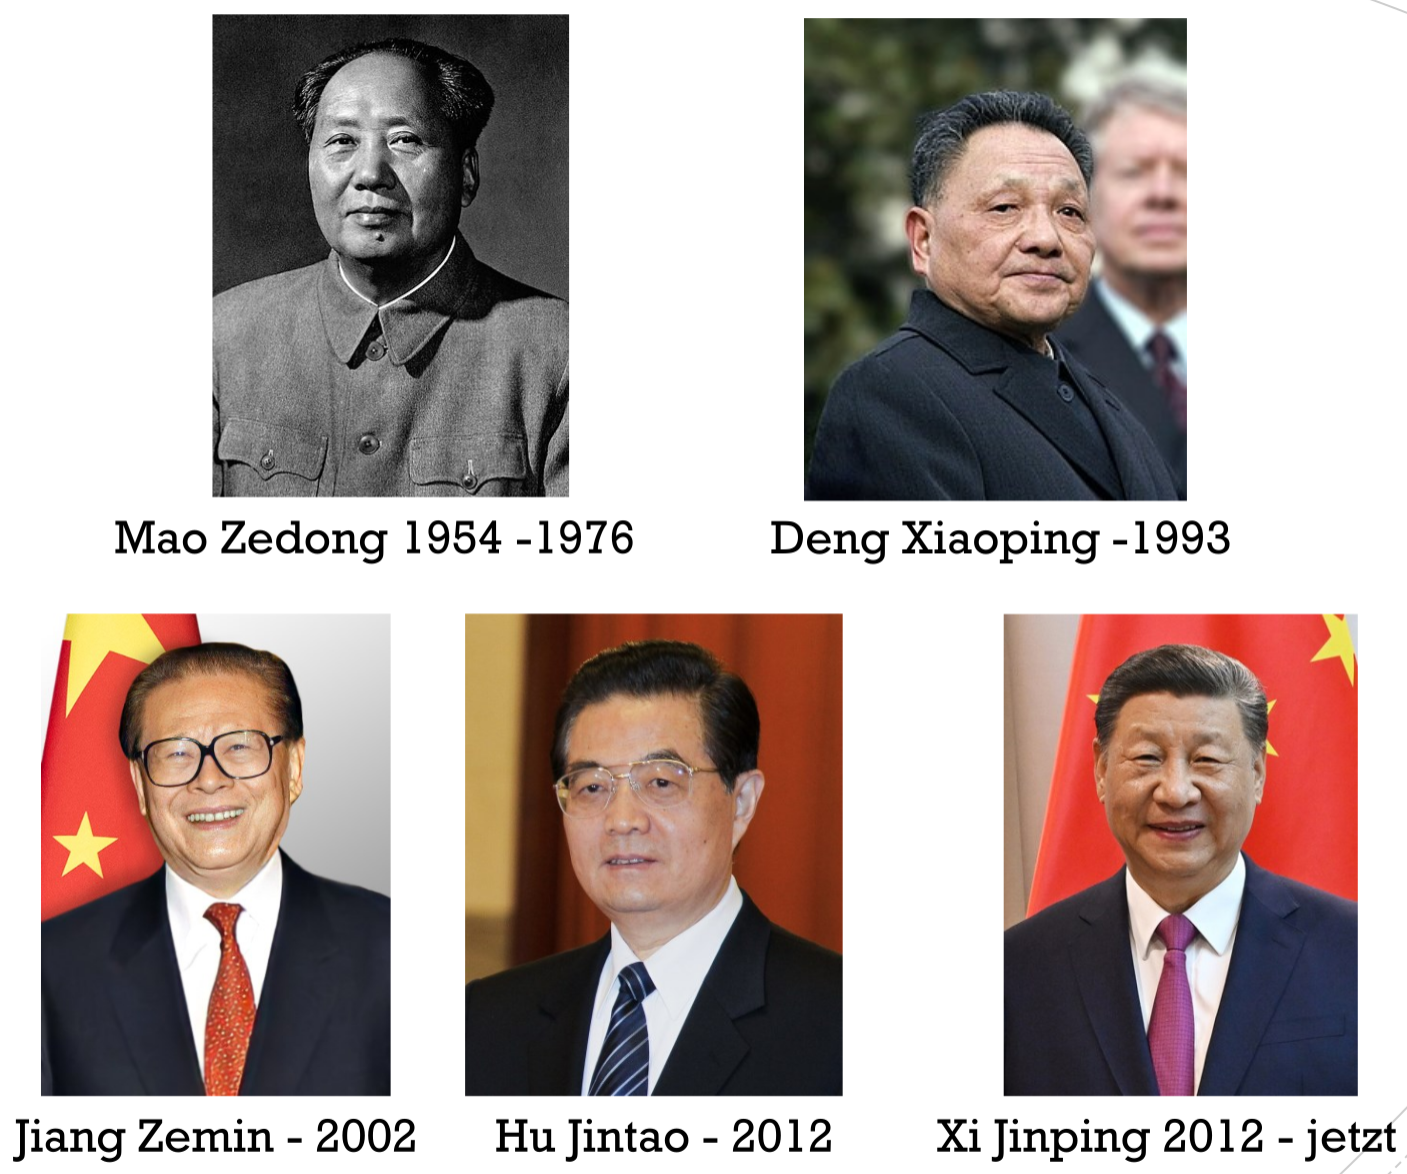
\includegraphics[width=\columnwidth]{images/kc.png}
		\caption{Bisherige Anführer Chinas}
	\end{figure}

	\subsection{PLA Modernisierung unter Xi Jinping}

	Verschlankung
	- PLA soll ``red'' und ``expert'' sein
	- Korruptionsbekämpfung
	- Besser Joint-Operations
	\textbf{Beispiele Material}
	- Type 055 Cruiser
	- Dongfeng 21 ``Carrier Killer''
	- Shenyang J-35 Kampfjet
	- Fuijan Flugzeugträger
	- Landebrückenschiffe
	- Drohnenträgerdrohnen

	\subsection{Militärstruktur Stand 2025}

	\textbf{Four Services}
	- Ground Force PLAGF (grün)
	- Navy PLAN (blau-weiss)
	- Air Force PLAAF (hellblau)
	- Rocket Force PLARF (gelb)

	\textbf{Four Arms (new)}
	- Aerospace Force
	- Cyberspace Force
	- Information Support
	- Joint Logistics Support

	\textbf{Weitere bewaffnete Verbände}
	- People's Armed Forces Militia (8 Millionen)
	- Peoples Armed Police (PAP) (1,5 Millionen)
	- Coast Guard



	\subsection{Krisen in der Taiwanstrasse}

	\begin{itemize}

		\item
		      1954 Taiwanstrassenkrise (Bomb. Kinmen und Matsu)
		\item
		      1958 2.Taiwanstrassenkrise (Luft- und Seegefechte)
		\item
		      1994 3.Taiwanstrassenkrise (Lee Teng-Hui in USA)
		\item
		      2022 4.Taiwanstrassenkrise (Nancy Pelosi in Taiwan)
	\end{itemize}


	\subsection{China Taiwan Vergleich}

	\begin{itemize}

		\item
		      Taiwan mit starken geographischen Vorteilen.
		\item
		      China qualitativ und quantitativ in allen Bereichen deutlich überlegen
		      aber Preis für Einnahme hoch.
	\end{itemize}


	\section{Sprechstunden}

	Sprechstundentermine können bei Bedarf individuell vereinbart werden.\\
	Bitte setzen Sie sich mit dem Dozenten in Verbindung:
	\href{mailto:marcel.berni@milak.ethz.ch}{\nolinkurl{marcel.berni@milak.ethz.ch}}

\end{multicols}

\end{document}
